\documentclass{article}
\usepackage[backend=biber,natbib=true,style=alphabetic,maxbibnames=10]{biblatex}
\addbibresource{/home/nqbh/reference/bib.bib}
\usepackage[utf8]{vietnam}
\usepackage{tocloft}
\renewcommand{\cftsecleader}{\cftdotfill{\cftdotsep}}
\usepackage[colorlinks=true,linkcolor=blue,urlcolor=red,citecolor=magenta]{hyperref}
\usepackage{amsmath,amssymb,amsthm,color,fancyvrb,float,graphicx,mathtools,multicol}
\usepackage{enumitem}
\setlist{leftmargin=4mm}
\setlength{\columnseprule}{.5pt}
\def\columnseprulecolor{\color{black}}
\allowdisplaybreaks
\newtheorem{assumption}{Assumption}
\newtheorem{baitoan}{Bài toán}
\newtheorem{cauhoi}{Câu hỏi}
\newtheorem{conjecture}{Conjecture}
\newtheorem{corollary}{Corollary}
\newtheorem{dangtoan}{Dạng toán}
\newtheorem{definition}{Definition}
\newtheorem{dinhly}{Định lý}
\newtheorem{dinhnghia}{Định nghĩa}
\newtheorem{example}{Example}
\newtheorem{ghichu}{Ghi chú}
\newtheorem{hequa}{Hệ quả}
\newtheorem{hypothesis}{Hypothesis}
\newtheorem{lemma}{Lemma}
\newtheorem{luuy}{Lưu ý}
\newtheorem{nhanxet}{Nhận xét}
\newtheorem{notation}{Notation}
\newtheorem{note}{Note}
\newtheorem{principle}{Principle}
\newtheorem{problem}{Problem}
\newtheorem{proposition}{Proposition}
\newtheorem{question}{Question}
\newtheorem{remark}{Remark}
\newtheorem{theorem}{Theorem}
\newtheorem{vidu}{Ví dụ}
\usepackage[left=1cm,right=1cm,top=5mm,bottom=5mm,footskip=4mm]{geometry}
\def\labelitemii{$\circ$}
\DeclareRobustCommand{\divby}{%
	\mathrel{\vbox{\baselineskip.65ex\lineskiplimit0pt\hbox{.}\hbox{.}\hbox{.}}}%
}

\title{Problems in Elementary Computer Science -- Bài Tập Tin Học Sơ Cấp}
\author{Nguyễn Quản Bá Hồng\footnote{e-mail: \texttt{nguyenquanbahong@gmail.com}, website: \url{https://nqbh.github.io}, Ben Tre City, Vietnam.}}
\date{\today}

\begin{document}
\maketitle

%------------------------------------------------------------------------------%

\begin{baitoan}[\cite{Huy_sang_tao_thuat_toan_lap_trinh_tap_1}, p. 6, số thân thiện -- friendly number]
	(a) Tìm tất cả các số tự nhiên có 2 chữ số mà khi đảo trật tự của 2 chữ số đó sẽ thu được 1 số nguyên tố cùng nhau với số đã cho. (b) Mở rộng $2$ thành $n\in\mathbb{N},n\ge2$.
\end{baitoan}

\begin{baitoan}[\cite{Huy_sang_tao_thuat_toan_lap_trinh_tap_1}, p. 13, cấp số cộng -- arithmetic progression]
	Tìm các số tự nhiên lẻ gồm 3 chữ số. 3 chữ số này, theo thứ tự từ trái qua phải tạo thành 1 cấp số cộng.
\end{baitoan}

\begin{baitoan}[\cite{Huy_sang_tao_thuat_toan_lap_trinh_tap_1}, p. 17, cấp số nhân -- geometric progression]
	Tìm các số tự nhiên gồm 3 chữ số. 3 chữ số này, theo thứ tự từ trái qua phải tạo thành 1 cấp số nhân với công bội $q\in\mathbb{N}^\star$.
\end{baitoan}

\begin{baitoan}[\cite{Trung_HSG_THPT_Tin}, 1., p. 13, HSG Lớp 10 Vĩnh Phúc 2020--2021, Square -- Hình vuông]
	(a) Cho $n$ điểm có tọa độ là các số nguyên trên hệ trục tọa độ $Oxy$. Tìm diện tích hình vuông nhỏ nhất có các cạnh song song với các trục tọa độ sao cho tất cả các điểm đã cho đều thuộc hình vuông đó (điểm nằm trên cạnh hình vuông cũng được coi là thuộc hình vuông đó).
	\begin{itemize}
		\item {\sf Input.} Dòng 1: chứa số nguyên dương $n\in\mathbb{N}^\star$, $2\le n\le20$, là số lượng điểm có tọa độ là các số nguyên. $n$ dòng tiếp theo, mỗi dòng ghi 2 số nguyên $x,y\in\mathbb{Z}$, $1\le x,y\le100$, là tọa độ của mỗi điểm.
		\item {\sf Output.} Ghi diện tích hình vuông nhỏ nhất tìm được.
		\item {\sf Sample.}
		\begin{table}[H]
			\centering
			\begin{tabular}{|l|l|}
				\hline
				{\tt square.inp} & {\tt square.out} \\
				\hline
				3 & 16 \\
				3 4 &  \\
				5 7 &  \\
				4 3 &  \\
				\hline
			\end{tabular}
		\end{table}
	\end{itemize}
	(b) Mở rộng bài toán từ `hình vuông' sang `hình chữ nhật', \& từ `tọa độ nguyên' sang `tọa độ thực': (i) Cho $n$ điểm có tọa độ là các số thực trên hệ trục tọa độ $Oxy$. Tìm diện tích hình vuông, hình vuông ``nguyên'', hình chữ nhật, \& hình chữ nhật ``nguyên'' nhỏ nhất có các cạnh song song với các trục tọa độ sao cho tất cả các điểm đã cho đều thuộc hình chữ nhật đó (điểm nằm trên cạnh hình chữ nhật cũng được coi là thuộc hình chữ nhật đó), trong đó {\rm hình vuông, hình chữ nhật ``nguyên''} lần lượt là các hình vuông \& hình chữ nhật có các tọa độ của 4 đỉnh là 8 số nguyên.
\end{baitoan}

\begin{baitoan}[\cite{Trung_HSG_THPT_Tin}, 2., pp. 13--14, HSG Lớp 10 Vĩnh Phúc 2020--2021, Divisible by 3 -- Chia hết cho 3]
	Cho dãy $a$ gồm $n$ số nguyên dương. Cho biết có bao nhiêu cặp số trong dãy có tổng chia hết cho $3$, i.e., đếm xem có bao nhiêu cặp chỉ số $i,j$, $1\le i < j\le n$, sao cho $a_i + a_j\divby3$.
	\begin{itemize}
		\item {\sf Input.} Dòng 1: 1 số nguyên duy nhất $n$, $1\le n\le10^5$. Dòng 2: Ghi $n$ số nguyên dương $a_1,a_2,\ldots,a_n$, $1\le a_i\le10^5$, $\forall i = 1,2,\ldots,n$, là các phần tử của dãy.
		\item {\sf Output.} 1 dòng duy nhất ghi số lượng cặp số của dãy $a$ có tổng chia hết cho $3$.
		\item {\sf Sample.}
		\begin{table}[H]
			\centering
			\begin{tabular}{|l|l|l|}
				\hline
				{\tt div3.inp} & {\tt div3.out} & Giải thích \\
				\hline
				5 & 3 & 3 cặp số tìm được có chỉ số: $(1,4),(2,3),(3,5)$. \\
				3 6 9 12 & & \\
				\hline
				4 & 6 & 6 cặp số tìm được có chỉ số: $(1,2),(1,3),(1,4),(2,3),(2,4),(3,4)$. \\
				3 6 9 12 & & \\
				\hline
			\end{tabular}
		\end{table}
	\end{itemize}
\end{baitoan}

\begin{baitoan}[\cite{Trung_HSG_THPT_Tin}, 3., p. 14, HSG Lớp 10 Vĩnh Phúc 2020--2021, Delete element -- Xóa phần tử]
	Cho dãy gồm $n$ số nguyên $a_1,a_2,\ldots,a_n$ với $1\le a_i\le3$, $\forall i = 1,2,\ldots,n$. Có bao nhiêu cách để xóa đi 1 số phần tử của dãy (không xóa phần tử nào cũng được coi là 1 cách) mà vẫn giữ nguyên thứ tự ban đầu để được 1 dãy mới thỏa mãn 2 yêu cầu sau: (i) Dãy còn ít nhất 3 phần  tử. (ii) Phần tử đầu tiên của dãy có giá trị $1$, tiếp theo là 1 số phần tử có giá trị là $2$ (ít nhất có 1 số $2$), \& kết thúc bằng đúng 1 phần tử có giá trị là $3$. E.g., các dãy $1,2,2,3$ \& $1,2,3$ thỏa mãn yêu cầu, các dãy $1,2,3,3$ \& $1,1,2,3$ không thỏa mãn yêu cầu.
	\begin{itemize}
		\item {\sf Input.} Dòng 1: 1 số nguyên dương $n\in\mathbb{N}^\star$, $n\le10^6$, là số lượng phần tử của dãy. Dòng 2: Ghi $n$ số nguyên dương $a_1,a_2,\ldots,a_n$ là giá trị của các phần tử của dãy ban đầu.
		\item {\sf Output.} Gồm 1 dòng duy nhất là số cách xóa để được dãy mới thỏa mãn yêu cầu của đề bài. Do số lượng cách xóa phần tử có thể rất lớn nên chỉ cần ghi ra số lượng cách xóa sau khi chia lấy dư cho $10^9 + 7$.
		\item {\sf Sample.}
		\begin{table}[H]
			\centering
			\begin{tabular}{|l|l|}
				\hline
				\verb|delete_element.inp| & \verb|delete_element.out| \\
				\hline
				8 & 15 \\
				1 2 1 2 3 1 2 3 &  \\
				\hline
			\end{tabular}
		\end{table}
	\end{itemize}
\end{baitoan}

\begin{baitoan}[\cite{Trung_HSG_THPT_Tin}, 1., p. 15, HSG Lớp 11 Vĩnh Phúc 2020--2021, Game button -- Trò chơi bấm nút]
	Người chơi đang tham gia 1 trò chơi như sau: Có 2 nút bấm A, B, trên nút A có ghi số $m_A$, trên nút B có ghi số $m_B$. Ở mỗi lượt chơi, người chơi phải chọn bấm 1 trong 2 nút \& sẽ nhận được số điểm thưởng bằng với số ghi trên nút đó, sau đó số trên nút bấm giảm đi $1$ đơn vị. Hỏi sau 2 lượt chơi, số điểm thưởng lớn nhất mà người chơi có thể nhận được là bao nhiêu?
	\begin{itemize}
		\item {\sf Input.} 1 dòng duy nhất ghi 2 số nguyên dương $m_A,m_B$ với $3\le A,B\le20$, tương ứng với 2 số ghi trên 2 nút A \& B.
		\item {\sf Output.} Ghi số điểm thưởng lớn nhất mà người chơi có thể nhận được sau 2 lượt chơi.
		\item {\sf Sample.}
		\begin{table}[H]
			\centering
			\begin{tabular}{|l|l|l|}
				\hline
				\verb|game_button.inp| & \verb|game_button.out| & Giải thích\\
				\hline
				5 3 & 9 & Bấm 2 lần nút A \& sẽ có tổng điểm thưởng: $5 + 4 = 9$. \\
				\hline
			\end{tabular}
		\end{table}
	\end{itemize}
\end{baitoan}

\begin{baitoan}[\cite{Trung_HSG_THPT_Tin}, 2., p. 15, HSG Lớp 11 Vĩnh Phúc 2020--2021, Count number -- Đếm số]
	Cho 4 số nguyên dương $a,b,c,d$. Đếm xem có bao nhiêu số nguyên dương $x\in\mathbb{N}^\star$ thỏa mãn các điều kiện sau: (i) $a\le x\le b$. (ii) $x\not{\divby}\ c$. (iii) $x\not{\divby}\ d$.
	\begin{itemize}
		\item {\sf Input.} 1 dòng duy nhất ghi 4 số $a,b,c,d$, $1\le a,b\le10^{18}$, $1\le c,d\le10^9$.
		\item {\sf Output.} 1 dòng duy nhất ghi số lượng số nguyên dương $x\in\mathbb{N}^\star$ thỏa mãn điều kiện đề bài.
		\item {\sf Sample.}
		\begin{table}[H]
			\centering
			\begin{tabular}{|l|l|l|}
				\hline
				\verb|count_number.inp| & \verb|count_number.out| & Giải thích \\
				\hline
				4 9 2 3 & 2 & Chỉ có số 5 \& 7 thỏa mãn điều kiện đề bài. \\
				\hline
			\end{tabular}
		\end{table}
	\end{itemize}
\end{baitoan}

\begin{baitoan}[\cite{Trung_HSG_THPT_Tin}, 3., p. 16, HSG Lớp 11 Vĩnh Phúc 2020--2021, Reverse \& reverse -- Lật qua lật lại]
	Cho dãy $a$ gồm $n\in\mathbb{N}^\star$ phần tử $1,2,\ldots,n$. Người ta thực hiện trên dãy số này đúng $k$ lần 2 thao tác sau: (i) Đầu tiên, đảo ngược thứ tự (lật đối xứng) đoạn phần tử có chỉ số từ $u$ đến $v$. (ii) Tiếp theo, đảo ngược thứ tự (lật đối xứng) đoạn phần tử có chỉ số từ $l$ đến $r$. Với $u,v,l,r$ là các hằng số cho trước. Đưa ra dãy $a$ sau khi thực hiện $k$ lần 2 thao tác nói trên.
	\begin{itemize}
		\item {\sf Input.} Dòng 1: 2 số nguyên dương $n,k\in\mathbb{N}^\star$, $1\le n\le100$, $1\le k\le10^9$. Dòng 2: gồm 2 số nguyên dương $u,v$, $1\le u < v\le n$. Dòng 3: gồm 2 số nguyên dương $l,r$, $1\le l < r\le n$.
		\item {\sf Output.} Ghi trên $n$ dòng, dòng thứ $i$ ghi giá trị của phần tử thứ $i$ của dãy $a$ sau khi thực hiện $k$ lần 2 thao tác nói trên, $\forall i = 1,2,\ldots,n$.
		\item {\sf Sample.}
		\begin{table}[H]
			\centering
			\begin{tabular}{|l|l|l|}
				\hline
				\verb|reverse_reverse.inp| & \verb|reverse_reverse.out| & Giải thích\\
				\hline
				7 2 & 1 & Dãy ban đầu: \\
				2 5 & 2 & 1 2 3 4 5 6 7 \\
				3 7 & 4 & Lần 1: \\
				& 3 & 1 \textit{5 4 3 2} 6 7 \\
				& 5 & 1 5 \textit{7 6 2 3 4} \\
				& 7 & Lần 2: \\
				& 6 & 1 \textit{2 6 7 5} 3 4 \\
				& & 1 2 4 3 5 7 6 \\
				\hline
			\end{tabular}
		\end{table}
	\end{itemize}
\end{baitoan}

\begin{baitoan}[\cite{Trung_HSG_THPT_Tin}, 3., p. 17, HSG Lớp 12 Vĩnh Phúc 2020--2021, Max gift -- Chọn quà mắc nhất]
	Cuối năm công ty tổ chức phát qua cho nhân viên. Có $n\in\mathbb{N}^\star$ gói quà với giá trị khác nhau được xếp liên tiếp thành 1 hàng, trong đó gói quà thứ $i$ có giá trị là $a_i$. Mỗi nhân viên chỉ được chọn 2 gói quà liên tiếp. Mr. Bean là người may mắn được chọn đầu tiên. Giúp Mr. Bean chọn ra 2 gói quà liên tiếp có giá trị lớn nhất.
	\begin{itemize}
		\item {\sf Input.} Dòng 1: chứa số nguyên dương $n\in\mathbb{N}^\star$, $2\le n\le10^6$. Dòng 2: Giá trị của $n$ gói quà, $1\le a_i\le10^3$, $\forall i = 1,2,\ldots,n$, mỗi giá trị cách nhau bởi dấu cách.
		\item {\sf Output.} 1 dòng duy nhất chứa tổng giá trị quà lớn nhất chọn được.
		\item {\sf Sample.}
		\begin{table}[H]
			\centering
			\begin{tabular}{|l|l|}
				\hline
				\verb|max_gift.inp| & \verb|max_gift.out| \\
				\hline
				5 & 9 \\
				1 3 5 4 2 &  \\
				\hline
			\end{tabular}
		\end{table}
	\end{itemize}
\end{baitoan}

\begin{baitoan}[\cite{Trung_HSG_THPT_Tin}, 2., pp. 17--18, HSG Lớp 12 Vĩnh Phúc 2020--2021, Decrease value -- Giảm giá trị]
	1 ngày rảnh rỗi, Mr. Bean chơi trò chơi với các con số. Mr. Bean lấy 1 số nguyên dương $n\in\mathbb{N}^\star$ rồi thực hiện không giới hạn số lần thao tác ``Chọn 1 chữ số $x$ của $n$ rồi giảm $n$ đi $x$ đơn vị''. Hỏi Mr. Bean phải thực hiện ít nhất bao nhiêu thao tác như vậy để giảm số $n$ về $0$. E.g., $n = 27$, Mr. Bean sẽ thực hiện 5 thao tác để biến đổi: (i) Chọn $x = 7\to n = 27 - 7 = 20$. (ii) Chọn $x = 2\to n = 20 - 2 = 18$. (iii) Chọn $x = 8\to n = 18 - 8 = 10$. (iv) Chọn $x = 1\to n = 10 - 1 = 9$. (v) Chọn $x = 9\to n = 9 - 9 = 0$.
	\begin{itemize}
		\item {\sf Input.} 1 dòng: 1 số nguyên dương duy nhất $n$, $1\le n\le10^6$.
		\item {\sf Output.} 1 dòng duy nhất ghi số thao tác ít nhất để biến đổi $n$ về $0$.
		\item {\sf Sample.}
		\begin{table}[H]
			\centering
			\begin{tabular}{|l|l|}
				\hline
				\verb|decrease_value.inp| & \verb|decrease_value.out| \\
				\hline
				27 & 5 \\
				\hline
			\end{tabular}
		\end{table}
	\end{itemize}
\end{baitoan}

\begin{baitoan}[\cite{Trung_HSG_THPT_Tin}, 3., p. 18, HSG Lớp 12 Vĩnh Phúc 2020--2021, Difference degree of substrings -- Xâu con phân biệt]
	1 lần Mr. Bean được bạn gái gửi cho 1 dãy ký tự $S$ độ dài $n$ chỉ gồm các chữ cái in hoa (`A',$\ldots$,`Z'). Bạn gái nhờ Mr. Bean xác định ``độ phân biệt'' của dãy ký tự trên. Trong đó {\rm độ phân biệt} của dãy ký tự là số nguyên dương $l$ nhỏ nhất sao cho tất cả các xâu con của $S$ độ dài $l$ là đôi một phân biệt. E.g., với $n = 7$, $S =$ `ABCDABC' thì $l = 4$ do tất cả các xâu con độ dài $4$ đều phân biệt. Giúp Mr. Bean việc đó.
	\begin{itemize}
		\item {\sf Input.} Dòng 1: số nguyên dương $n\in\mathbb{N}^\star$, $n\le100$. Dòng 2: chứa xâu ký tự S.
		\item {\sf Output.} Gồm 1 dòng duy nhất ghi 1 số nguyên duy nhất là ``độ phân biệt'' của dãy ký tự S.
		\item {\sf Sample.}
		\begin{table}[H]
			\centering
			\begin{tabular}{|l|l|}
				\hline
				\verb|diff_substring.inp| & \verb|diff_substring.out| \\
				\hline
				7 & 4 \\
				ABCDABC &  \\
				\hline
			\end{tabular}
		\end{table}
	\end{itemize}
\end{baitoan}

\begin{baitoan}[\cite{Trung_HSG_THPT_Tin}, 4., p. 18, HSG Lớp 12 Vĩnh Phúc 2020--2021, Ants meet -- Kiến tha mồi]
	Trên đường đi làm về Mr. Bean quan sát thấy 2 ổ kiến cách nhau 1 khoảng $l$ đơn vị. Các con kiến đang tha mồi về 2 tổ trên đường thẳng nối 2 tổ kiến với nhau. Các con kiến khi tha mồi về tổ nào thì ở lại tổ đó. Nếu 2 con kiến gặp nhau trên đường đi thì cả 2 sẽ đổi hướng di chuyển.
	
	Giả sử đường nối giữa 2 tổ kiến được gắn tọa độ từ $0$ đến $l$. Tổ thứ nhất ở vị trí $0$ \& tổ thứ 2 ở vị trí $l$. Ở thời điểm Mr. Bean quan sát có $n$ con kiến đang tha mồi về tổ. Con thứ $i$ xuất phát ở tọa độ $x_i$, mang lượng mồi khối lượng $w_i$ \& có hướng di chuyển $d_i$. Nếu $d_i = 1$ thì con kiến thứ $i$ đang di chuyển theo hướng $0$ về $l$, $d_i = -1$ thì con kiến thứ $i$ đang di chuyển theo chiều ngược lại. Tất cả các con kiến có tốc độ di chuyển bằng nhau \& bằng $1$ đơn vị đo độ dài trên giây.
	
	Gọi $t$ là thời điểm sớm nhất tính từ thời điểm quan sát mà tổng lượng mồi được tha về 2 tổ đạt ít nhất $\frac{1}{2}$ tổng lượng mồi của đàn kiến. Mr. Bean đếm được trong thời gian đó các con kiến gặp nhau đúng $x$ lần, tính cả lần gặp nhau ở thời điểm $t$. Hỏi $x$ bằng bao nhiêu?
	\begin{itemize}
		\item {\sf Input.} Dòng 1: 2 số nguyên dương $n,l\in\mathbb{N}^\star$, $1\le n\le5\cdot10^4$, $1\le l\le10^9$. Dòng 2,$\ldots,n + 1$: Dòng $i + 1$ ghi 3 số nguyên $w_i,x_i,d_i$, $1\le w_i\le10^3$, $d_i = \pm1$, $0\le x_i\le l$, các số $x_i$, $i = 1,2,\ldots,n$, đôi một phân biệt. Các số nguyên cách nhau 1 dấu cách.
		\item {\sf Output.} 1 dòng duy nhất chứa số nguyên $x\in\mathbb{N}^\star$ là số lần gặp nhau của các cặp kiến.
		\item {\sf Sample.}
		\begin{table}[H]
			\centering
			\begin{tabular}{|l|l|}
				\hline
				\verb|ant_meet.inp| & \verb|ant_meet.out| \\
				\hline
				3 5 & 2 \\
				1 1 1 & \\
				2 2 -1 & \\
				3 3 -1 & \\
				\hline
			\end{tabular}
		\end{table}
		Giải thích: Thời điểm $0.5$, kiến 1 gặp kiến 2 ở tọa độ $1.5$, kiến 1 đổi hướng thành $-1$, kiến 2 đổi hướng thành $1$. Thời điểm 1, kiến 2 gặp kiến 3 ở tọa độ $2$, kiến 2 đổi hướng thành $-1$, kiến 3 đổi hướng thành $1$. Thời điểm 2: kiến 1 về đến tổ ở tọa độ $0$. Thời điểm 3: kiến 2 về đến tổ ở tọa độ $0$, lúc này lượng mồi đạt được ở 2 tổ là $3$, bằng  $\frac{1}{2}$ tổng lượng mồi của cả 3 kiến.
	\end{itemize}
\end{baitoan}

\begin{baitoan}[\cite{Trung_HSG_THPT_Tin}, 1., p. 20, HSG Lớp 12 Nam Định 2020--2021, Nearly perfect number -- Số gần hoàn hảo]
	1 số nguyên dương $a\in\mathbb{N}^\star$ được gọi là {\rm số ``gần hoàn hảo''} nếu thỏa mãn điều kiện: $2a\le k$ với $k$ là tổng các ước số của $a$, e.g., $12$ là 1 số ``gần hoàn hảo'' vì $2\cdot12 < 1 + 2 + 3 + 4 + 6 + 12$ ($24 < 28$).
	\begin{itemize}
		\item {\sf Input.} Dòng đầu tiên chứa số nguyên dương $n\in\mathbb{N}^\star$, $1\le n\le10^4$. $n$ dòng tiếp theo, mỗi dòng là 1 số nguyên dương có giá trị $\le10^6$.
		\item {\sf Output.} Dòng đầu tiên ghi số lượng số ``gần hoàn hảo''. Các dòng tiếp theo, mỗi dòng ghi 1 số ``gần hoàn hảo'', số gặp trước thì viết trước.
		\item {\sf Sample.}
		\begin{table}[H]
			\centering
			\begin{tabular}{|l|l|}
				\hline
				\verb|near_perfect_number.inp| & \verb|near_perfect_number.out| \\
				\hline
				5 & 2 \\
				8 & 12 \\
				16 & 6 \\
				12 & \\
				6 & \\
				7 & \\
				\hline
			\end{tabular}
		\end{table}
	\end{itemize}
\end{baitoan}

\begin{baitoan}[\cite{Trung_HSG_THPT_Tin}, 2., pp. 20--21, HSG Lớp 12 Nam Định 2020--2021, Special number -- Số đặc biệt]
	Cho 1 dãy gồm $n$ số nguyên $a_1,a_2,\ldots,a_n$. Đếm \& đưa ra số đặc biệt trong dãy $a$. {\rm Số đặc biệt} là số chỉ xuất hiện đúng 1 lần trong dãy số.
	\begin{itemize}
		\item {\sf Input.} Dòng đầu tiên là số $n\in\mathbb{N}^\star$, $1\le n\le10^6$. $n$ dòng tiếp theo, dòng thứ $i$ là số $a_i$, $|a_i|\le10^9$, $\forall i = 1,2,\ldots,n$.
		\item {\sf Output.} Dòng đầu tiên ghi số lượng số đặc biệt. Các dòng tiếp theo, mỗi dòng ghi 1 số đặc biệt tính từ đầu dãy $a$.
		\item {\sf Sample.}
		\begin{table}[H]
			\centering
			\begin{tabular}{|l|l|}
				\hline
				\verb|special_number.inp| & \verb|special_number.out| \\
				\hline
				8 & 3 \\
				9 & 6 \\
				9 & 11 \\
				7 & 5 \\
				7 & \\
				6 & \\
				11 & \\
				9 & \\
				5 & \\
				\hline
			\end{tabular}
		\end{table}
	\end{itemize}
\end{baitoan}

\begin{baitoan}[\cite{Trung_HSG_THPT_Tin}, 3., p. 21, HSG Lớp 12 Nam Định 2020--2021, Game of gifts -- Trò chơi tặng quà]
	1 công ty có tổ chức trò chơi, tặng $n\in\mathbb{N}^\star$ gói quà đã được chuẩn bị theo giá trị phần quà từ thấp đến cao, để tri ân cho $n$ khách hàng. Công ty đó đã chuẩn bị 1 chiếc hộp đựng $n$ mảnh giấy, mỗi mảnh giấy được bí mật ghi 1 mã hóa gồm nhiều ký tự số \& chữ. Mỗi khách hàng được chọn 1 mảnh giấy trong chiếc hộp đó. Viết chương trình tặng quà từ thấp đến cao theo số lượng các ký tự số của mã hóa trong tờ giấy, nếu số lượng ký tự số trong mã hóa bằng nhau thì khách hàng chọn trước được tặng quà trước.
	\begin{itemize}
		\item {\sf Input.} Dòng đầu tiên chứa số nguyên dương $n\in\mathbb{N}^\star$, $1\le n\le10^4$. $n$ dòng tiếp theo, mỗi dòng chứa 1 mã hóa không dài quá $255$ ký tự tương ứng cho từng khách hàng.
		\item {\sf Output.} Thứ tự tặng quà của trò chơi này cho $n$ khách hàng trên.
		\item {\sf Sample.}
		\begin{table}[H]
			\centering
			\begin{tabular}{|l|l|}
				\hline
				\verb|game_gift.inp| & \verb|game_gift.out| \\
				\hline
				5 & G2Chuc \\
				N123456Cao & A89Dat \\
				A89Dat & L512Ket \\
				G2Chuc & E3689Qua \\
				L512Ket & N123456Cao \\
				E3689Qua &  \\
				\hline
			\end{tabular}
		\end{table}
	\end{itemize}
\end{baitoan}

\begin{baitoan}[\cite{Trung_HSG_THPT_Tin}, 4., pp. 21--22, HSG Lớp 12 Nam Định 2020--2021, Work -- Công việc]
	Trong 1 dây chuyền làm việc của công ty có $n$ công nhân làm $n$ việc. Người ta đánh số cho công nhân từ $1$ đến $n$ theo thứ tự đứng trong dây chuyền. Thời gian hoàn thành 1 công việc của người thứ $i$ là $t_i$ phút. Mỗi người cần làm xong công việc của mình nhưng được quyền làm tối đa $2$ việc. Vì thế họ có thể phối hợp với người đứng ngay trước mình cùng làm, nếu người thứ $i$ \& người thứ $i + 1$ phối hợp thì thời gian làm xong việc cho $2$ người là $p_i$. Tìm phương án sao cho $n$ công việc đều hoàn thành với thời gian ít nhất.
	\begin{itemize}
		\item {\sf Input.} Dòng 1 ghi số $n$, $1 < n\le10^6$. Dòng 2 ghi thời gian làm xong việc của từng công nhân tương ứng trong dây chuyền $t_1,t_2,\ldots,t_n$, $1\le t_i\le60$, $\forall i = 1,2,\ldots,n$. Dòng 3 ghi $n - 1$ số thời gian cùng làm tương ứng cho số cặp công nhân nếu phối hợp $p_1,p_2,\ldots,p_{n-1}$, $1\le p_i\le100$, $\forall i = 1,2,\ldots,n$.
		\item {\sf Output.} 1 số duy nhất ghi tổng thời gian hoàn thành công việc ít nhất của $n$ công nhân.
		\item {\sf Sample.}
		\begin{table}[H]
			\centering
			\begin{tabular}{|l|l|}
				\hline
				\verb|work.inp| & \verb|work.out| \\
				\hline
				5 & 17 \\
				2 5 7 8 4 & \\
				3 9 10 10 & \\
				\hline
			\end{tabular}
		\end{table}
	\end{itemize}
\end{baitoan}

%------------------------------------------------------------------------------%

\section{CSES Problem Set}

\subsection{Introductory Problems}

\begin{problem}[Weird Algorithm]
	Consider an algorithm that takes as input a positive integer $n\in\mathbb{N}^\star$. If $n$ is even, the algorithm divides it by $2$, \& if $n$ is odd, the algorithm multiplies it by $3$ \& adds $1$. The algorithms repeats this, until $n$ is $1$. E.g., the sequence for $n = 3$ is as follows: $3\to10\to5\to16\to8\to4\to2\to1$. Your task is to simulate the execution of the algorithm for a given value of $n$.
	\begin{itemize}
		\item {\sf Input.} The only input line contains an integer $n\in\mathbb{Z}$.
		\item {\sf Output.} Print a line that contains all values of $n$ during the algorithm.
		\item {\sf Constraints.} $1\le n\le10^6$.
		\item {\sf Sample.}
		\begin{table}[H]
			\centering
			\begin{tabular}{|l|l|}
				\hline
				\verb|weird_algorithm.inp| & \verb|weird_algorithm.out| \\
				\hline
				3 & 3 10 5 16 8 4 2 1 \\
				\hline
			\end{tabular}
		\end{table}
	\end{itemize}
\end{problem}
Source: \href{https://cses.fi/problemset/task/1068}{CSES Problem Set{\tt/}weird algorithm}, \& \cite[Sect. 1.3, pp. 5--7]{Laaksonen2020}.

\begin{problem}[Missing Number]
	You are given all numbers between $1,2,\ldots,n$ except one. Your task is to find the missing number.
	\begin{itemize}
		\item {\sf Input.} The 1st input line contains a positive integer $n\in\mathbb{N}^\star$. The 2nd line contains $n - 1$ numbers. Each number is distinct \& between $1$ \& $n$ (inclusive).
		\item {\sf Output.} Print the missing number.
		\item {\sf Constraints.} $2\le n\le2\cdot10^5$.
		\item {\sf Sample.}
		\begin{table}[H]
			\centering
			\begin{tabular}{|l|l|}
				\hline
				\verb|missing_number.inp| & \verb|missing_number.out| \\
				\hline
				5 & 4 \\
				2 3 1 5 & \\
				\hline
			\end{tabular}
		\end{table}
	\end{itemize}
\end{problem}
Source: \href{https://cses.fi/problemset/task/1083}{CSES Problem Set{\tt/}missing number}.

\begin{problem}[Repetitions]
	You are given a DNA sequence: a string consisting of characters A, C, G, \& T. Your task is to find the longest repetition in the sequence. This is a maximum-length substring containing only 1 type of character.
	\begin{itemize}
		\item {\sf Input.} The only input line contains a string of $n\in\mathbb{N}^\star$ characters.
		\item {\sf Output.} Print 1 integer: the length of the longest repetition.
		\item {\sf Constraints.} $1\le n\le10^6$.
		\item {\sf Sample.}
		\begin{table}[H]
			\centering
			\begin{tabular}{|l|l|}
				\hline
				\verb|repetition.inp| & \verb|repetition.out| \\
				\hline
				ATTCGGGA & 3 \\
				\hline
			\end{tabular}
		\end{table}
	\end{itemize}	
\end{problem}
Source: \href{https://cses.fi/problemset/task/1069}{CSES problem Set{\tt/}repetition}.

\begin{problem}[Nondecreasing Array]
	You are given an array of $n$ integers. You want to modify the array so that it is non-decreasing, i.e., every element is at least as large as the previous element. On each move, you may increase the value of any element by $1$. What is the minimum number of moves required?
	\begin{itemize}
		\item {\sf Input.} The 1st input line contains an integer $n$: the size of the array. The 2nd line contains $n$ integers $x_1,x_2,\ldots,x_n$: the contents of the array.
		\item {\sf Output.} Print the minimum number of moves.
		\item {\sf Constraints.} $1\le n\le2\cdot10^5$, $1\le x_i\le10^9$.
		\item {\sf Sample.}
		\begin{table}[H]
			\centering
			\begin{tabular}{|l|l|}
				\hline
				\verb|nondecreasing_array.inp| & \verb|nondecreasing_array.out| \\
				\hline
				5 & 5 \\
				3 2 5 1 7 & \\
				\hline
			\end{tabular}
		\end{table}
	\end{itemize}
\end{problem}
Source: \href{https://cses.fi/problemset/task/1094}{CSES problem Set{\tt/}increasing array}.

\begin{problem}[Permutations]
	A permutation of integers $1,2,\ldots,n$ is called \emph{beautiful} if there are no adjacent elements whose difference is $1$. Given $n$, construct a beautiful permutation if such a permutation exists.
	\begin{itemize}
		\item {\sf Input.} The only input line contains an integer $n$.
		\item {\sf Output.} Print a beautiful permutation of integers $1,2,\ldots,n$. If there are several solutions, you may print any of them. If there are no solutions, print \verb|"no solution"|.
		\item {\sf Constraints.} $1\le n\le10^6$.
		\item {\sf Sample.}
		\begin{table}[H]
			\centering
			\begin{tabular}{|l|l|}
				\hline
				\verb|permutations.inp| & \verb|permutations.out| \\
				\hline
				5 & 4 2 5 3 1 \\
				\hline
				3 & NO SOLUTION \\
				\hline
			\end{tabular}
		\end{table}
	\end{itemize}
\end{problem}
Source: \href{https://cses.fi/problemset/task/1070}{CSES problem Set{\tt/}permutations}.

\begin{problem}[Number Spiral]
	A \emph{number spiral} is an infinite grid whose upper-left square has number $1$. Here are the 1st 5 layers of the spiral:
	\begin{table}[H]
		\centering
		\begin{tabular}{|c|c|c|c|c|}
			\hline
			1 & 2 & 9 & 10 & 25 \\
			\hline
			4 & 3 & 8 & 11 & 24 \\
			\hline
			5 & 6 & 7 & 12 & 23 \\
			\hline
			16 & 15 & 14 & 13 & 22 \\
			\hline
			17 & 18 & 19 & 20 & 21 \\
			\hline
		\end{tabular}
	\end{table}
	Your task is to find out the number in row $y$ \& column $x$.
	\begin{itemize}
		\item {\sf Input.} The 1st input line contains an integer $t$: the number of tests. After this, there are $t$ lines, each containing integers $y,x$.
		\item {\sf Output.} For each test, print the number in row $y$ \& column $x$.
		\item {\sf Constraints.} $1\le t\le10^5$, $1\le x,y\le10^9$.
		\item {\sf Sample.}
		\begin{table}[H]
			\centering
			\begin{tabular}{|l|l|}
				\hline
				\verb|number_spiral.inp| & \verb|number_spiral.out| \\
				\hline
				3 & 8 \\
				2 3 & 1 \\
				1 1 & 15 \\
				4 2 & \\
				\hline				
			\end{tabular}
		\end{table}
	\end{itemize}
\end{problem}
Source: \href{https://cses.fi/problemset/task/1071}{CSES problem Set{\tt/}number spiral}.

\begin{problem}[2 Knights]
	Your task is to count for $k = 1,2,\ldots,n$ the number of ways 2 knights can be placed on a $k\times k$ chessboard so that they do not attack each other.
	\begin{itemize}
		\item {\sf Input.} The only input line contains a positive integer $n\in\mathbb{N}^\star$.
		\item {\sf Output.} Print $n$ integers: the results.
		\item {\sf Constraints.} $1\le n\le10^4$.
		\item {\sf Sample.}
		\begin{table}[H]
			\centering
			\begin{tabular}{|l|l|}
				\hline
				\verb|knight.inp| & \verb|knight.out| \\
				\hline
				8 & 0 \\
				& 6 \\
				& 28 \\
				& 96 \\
				& 252 \\
				& 550 \\
				& 1056 \\
				& 1048 \\
				\hline
			\end{tabular}
		\end{table}
	\end{itemize}
\end{problem}
Source: \href{https://cses.fi/problemset/task/1072}{CSES problem Set{\tt/}2 knights}.

\begin{problem}[2 Sets]
	Your task is to divide the numbers $1,2,\ldots,n$ into 2 sets of equal sum.
	\begin{itemize}
		\item {\sf Input.} The only input line contains a positive integer $n\in\mathbb{N}^\star$.
		\item {\sf Output.} Print ``yes'', if the division is possible, \& ``no'' otherwise. After this, if the division is possible, print an example of how to create the sets. 1st, print the number of elements in the 1st set followed by the elements themselves in a separate line, \& then, print the 2nd set in a similar way.
		\item {\sf Constraints.} $1\le n\le10^6$.
		\item {\sf Sample.}
		\begin{table}[H]
			\centering
			\begin{tabular}{|l|l|}
				\hline
				\verb|set2.inp| & \verb|set2.out| \\
				\hline
				7 & yes \\
				& 4 \\
				& 1 2 4 7 \\
				& 3 \\
				& 3 5 6 \\
				\hline
				6 & no \\
				\hline
			\end{tabular}
		\end{table}
	\end{itemize}
\end{problem}
Source: \href{https://cses.fi/problemset/task/1092}{CSES problem Set{\tt/}2 sets}.

\begin{problem}[Bit String]
	Your task is to calculate the number of bit strings of length $n$. E.g., if $n = 3$, the correct answer is $8$, because the possible bit strings are {\tt000, 001, 010, 011, 100, 101, 110}, \& {\tt111}.
	\begin{itemize}
		\item {\sf Input.} The only input line contains a positive integer $n\in\mathbb{N}^\star$.
		\item {\sf Output.} Print the result modulo $10^9 + 7$.
		\item {\sf Constraints.} $1\le n\le10^6$.
		\item {\sf Sample.}
		\begin{table}[H]
			\centering
			\begin{tabular}{|l|l|}
				\hline
				\verb|bit_string.inp| & \verb|bit_string.out| \\
				\hline
				3 & 8 \\
				\hline
			\end{tabular}
		\end{table}
	\end{itemize}
\end{problem}
Source: \href{https://cses.fi/problemset/task/1617}{CSES problem Set{\tt/}bit string}.

\begin{problem}[Trailing Zeros]
	Your task is to calculate the number of trailing zeros in the factorial $n!$, e.g., $20! = 2432902008176640000$ \& it has $4$ trailing zeroes.
	\begin{itemize}
		\item {\sf Input.} The only input line contains a positive integer $n\in\mathbb{N}^\star$.
		\item {\sf Output.} Print the number of trailing zeros in $n!$.
		\item {\sf Constraints.} $1\le n\le10^9$.
		\item {\sf Sample.}
		\begin{table}[H]
			\centering
			\begin{tabular}{|l|l|}
				\hline
				\verb|trailing_zero.inp| & \verb|trailing_zero.out| \\
				\hline
				20 & 4 \\
				\hline
			\end{tabular}
		\end{table}
	\end{itemize}
\end{problem}
Source: \href{https://cses.fi/problemset/task/1618}{CSES problem Set{\tt/}trailing zeroes}.

\begin{problem}[Coin Piles]
	You have 2 coin piles containing $a$ 
	\& $b$ coins. On each move, you can either remove 1 coin from the left pile \& 2 coins from the right pile, or 2 coins from the left pile \& 1 coin from the right pile. Your task is to efficiently find out if you can empty both the piles.
	\begin{itemize}
		\item {\sf Input.} The 1st input line has an integer $t$: the number of tests. After this, there are $t$ lines, each of which has 2 integers $a$ \& $b$: the numbers of coins in the piles.
		\item {\sf Output.} For each test, print ``yes'' if you can empty the piles \& ``no'' otherwise.
		\item {\sf Constraints.} $1\le t\le10^5$, $0\le a,b\le10^9$.
		\item {\sf Sample.}
		\begin{table}[H]
			\centering
			\begin{tabular}{|l|l|}
				\hline
				\verb|max_gift.inp| & \verb|max_gift.out| \\
				\hline
				3 & yes \\
				2 1 & no \\
				2 2 & yes \\
				3 3 & \\
				\hline
			\end{tabular}
		\end{table}
	\end{itemize}
\end{problem}
Source: \href{https://cses.fi/problemset/task/1754}{CSES problem Set{\tt/}coin piles}.

\begin{problem}[Palindrome Reorder]
	Given a string, your task is to reorder its letters in such a way that it becomes a palindrome (i.e., it reads the same towards \& backwards).
	\begin{itemize}
		\item {\sf Input.} The only input line has a string of length $n$ consisting of characters A-Z.
		\item {\sf Output.} Print a palindrome consisting of the characters of the original string. You may print any valid solution. If there are no solutions, print ``no solution''.
		\item {\sf Constraints.} $1\le n\le10^6$.
		\item {\sf Sample.}
		\begin{table}[H]
			\centering
			\begin{tabular}{|l|l|}
				\hline
				\verb|palindrome_reorder.inp| & \verb|palindrome_reorder.out| \\
				\hline
				AAAACACBA & AACABACAA \\
				\hline
			\end{tabular}
		\end{table}
	\end{itemize}
\end{problem}
Source: \href{https://cses.fi/problemset/task/1755}{CSES problem Set{\tt/}palindrome reorder}.

\begin{problem}[Gray Code]
	A Gray code is a list of all $2^n$ bit strings of length $n$, where any 2 successive strings differ in exactly 1 bit (i.e., their Hamming distance is $1$). Your task is to create a Gray code for a given length $n$.
	\begin{itemize}
		\item {\sf Input.} The only input line has a positive integer $n\in\mathbb{N}^\star$.
		\item {\sf Output.} Print $2^n$ lines that describe the Gray code. You can print any valid solution.
		\item {\sf Constraints.} $1\le n\le10^6$.
		\item {\sf Sample.}
		\begin{table}[H]
			\centering
			\begin{tabular}{|l|l|}
				\hline
				\verb|gray_code.inp| & \verb|gray_code.out| \\
				\hline
				2 & 00 \\
				& 01 \\
				& 11 \\
				& 10 \\
				\hline
			\end{tabular}
		\end{table}
	\end{itemize}
\end{problem}
Source: \href{https://cses.fi/problemset/task/2205}{CSES problem Set{\tt/}gray code}.

\begin{problem}[Tower of Hà Nội]
	The Tower of Hanoi game consists of 3 stacks (left, middle, \& right) \& $n$ round disks of different sizes. Initially, the left stack has all the disks, in increasing order of size from top to bottom. The goal is to move all the disks to the right stack using the middle stack. On each move you can move the uppermost disk from a stack to another stack. In addition, it is not allowed to place a larger disk on a smaller disk. Your task is to find a solution that minimizes the number of moves.
	\begin{itemize}
		\item {\sf Input.} The only input line has a positive integer$n\in\mathbb{N}^\star$: the number of disks.
		\item {\sf Output.} 1st print a positive integer $k\in\mathbb{N}^\star$: the minimum number of moves. After this, print $k$ lines that describe the moves. Each line has 2 integers $a,b\in\{1,2,3\}$: you move a disk from stack $a$ to stack $b$.
		\item {\sf Constraints.} $1\le n\le16$.
		\item {\sf Sample.}
		\begin{table}[H]
			\centering
			\begin{tabular}{|l|l|}
				\hline
				\verb|.inp| & \verb|.out| \\
				\hline
				2 & 3 \\
				& 1 2 \\
				& 1 3 \\
				& 2 3 \\
				\hline
			\end{tabular}
		\end{table}
	\end{itemize}
\end{problem}
Source: \href{https://cses.fi/problemset/task/2165}{CSES problem Set{\tt/}tower of Hà Nội}.

\begin{problem}[Creating Strings]
	Given a string, your task is to generate all different strings that can be created using its characters.
	\begin{itemize}
		\item {\sf Input.} The only input line has a string of length $n\in\mathbb{N}^\star$. Each character is between a--z.
		\item {\sf Output.} 1st print a positive integer $k\in\mathbb{N}^\star$: the number of strings. Then print $k$ lines: the strings in alphabetical order.		
		\item {\sf Constraints.} $1\le n\le8$.
		\item {\sf Sample.}
		\begin{table}[H]
			\centering
			\begin{tabular}{|l|l|}
				\hline
				\verb|create_string.inp| & \verb|create_string.out| \\
				\hline
				aabac & 20 \\
				& aaabc \\
				& aaacb \\
				& aabac \\
				& aabca \\
				& aacab \\
				& aacba \\
				& abaac \\
				& abaca \\
				& abcaa \\
				& acaab \\
				& acaba \\
				& acbaa \\
				& baaac \\
				& baaca \\
				& bacaa \\
				& bcaaa \\
				& caaab \\
				& caaba \\
				& cabaa \\
				& cbaaa \\
				\hline
			\end{tabular}
		\end{table}
	\end{itemize}
\end{problem}
Source: \href{https://cses.fi/problemset/task/1622}{CSES problem Set{\tt/}creating strings}.

\begin{problem}[Apple Division]
	There are $n$ apples with known weights. Your task is to divide the apples into 2 groups so that the difference between the weights of the groups is minimal.
	\begin{itemize}
		\item {\sf Input.} The first input line has an integer $n\in\mathbb{N}^\star$: the number of apples. The next line has $n$ integers $p_1,p_2,\ldots,p_n$: the weight of each apple.
		\item {\sf Output.} Print 1 integer: the minimum difference between the weights of the groups.
		\item {\sf Constraints.} $1\le n\le20$, $1\le p_i\le10^9$.
		\item {\sf Sample.}
		\begin{table}[H]
			\centering
			\begin{tabular}{|l|l|}
				\hline
				\verb|apple_division.inp| & \verb|apple_division.out| \\
				\hline
				5 & 1 \\
				3 2 7 4 1 &  \\
				\hline
			\end{tabular}
		\end{table}
		Explanation: Group 1 has weights $2,3,4$ (total weight $9$), \& group 2 has weights $1$ \& $7$ (total weight $8$).
	\end{itemize}
\end{problem}
Source: \href{https://cses.fi/problemset/task/1623}{CSES problem Set{\tt/}apple division}.

\begin{problem}[Chessboard \& Queens]
	Your task is to place 8 queens on a chessboard so that no 2 queens are attacking each other. As an additional challenge, each square is either free or reserved, \& you can only place queens on the free squares. However, the reserved squares do not prevent queens from attacking each other. How many possible ways are there to place the queens?	
	\begin{itemize}
		\item {\sf Input.} The input has 8 lines, and each of them has 8 characters. Each square is either free (.) or reserved (*).
		\item {\sf Output.} Print 1 integer: the number of ways you can place the queens.
		\item {\sf Sample.} Input:
\begin{verbatim}
........
........
..*.....
........
........
.....**.
...*....
........
\end{verbatim}
		Output: $65$
	\end{itemize}
\end{problem}
Source: \href{https://cses.fi/problemset/task/1624}{CSES problem Set{\tt/}chessboard \& queens}.

\begin{problem}[Digit Queries]
	Consider an infinite string that consists of all positive integers in increasing order:
	\begin{align*}
		123456789101112131415161718192021222324252627282930\ldots
	\end{align*}
	Your task is to process $q$ queries of the form: what is the digit at position $k$ in the string?
	\begin{itemize}
		\item {\sf Input.} The 1st input line has a positive integer $q\in\mathbb{N}^\star$: the number of queries. After this, there are $q$ lines that describe the queries. Each line has an integer $k$: a 1-indexed position in the string.
		\item {\sf Output.} For each query, print the corresponding digit.
		\item {\sf Constraints.} $1\le q\le1000$, $1\le k\le10^{18}$.
		\item {\sf Sample.}
		\begin{table}[H]
			\centering
			\begin{tabular}{|l|l|}
				\hline
				\verb|digit_query.inp| & \verb|digit_query.out| \\
				\hline
				3 & 7 \\
				7 & 4 \\
				19 & 1 \\
				12 & \\
				\hline
			\end{tabular}
		\end{table}
	\end{itemize}
\end{problem}
Source: \href{https://cses.fi/problemset/task/2431}{CSES problem Set{\tt/}digit queries}.

\begin{problem}[Grid Path]
	There are $88418$ paths in a $7\times7$ grid from the upper-left square to the lower-left square. Each path corresponds to a $48$-character description consisting of characters {\tt D} (down), {\tt U} (up), {\tt L} (left), \& {\tt R} (right). E.g., the path
	\begin{figure}[H]
		\centering
		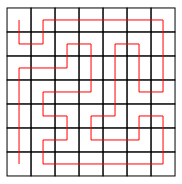
\includegraphics[scale=.5]{grid_path}
	\end{figure}
	\noindent corresponds to the description {\tt DRURRRRRDDDLUULDDDLDRRURDDLLLLLURULURRUULDLLDDDD}. You are given a description of a path which may also contain characters {\tt?} (any direction). Your task is to calculate the number of paths that match the description.
	\begin{itemize}
		\item {\sf Input.} The only input line has a $48$-character string of characters {\tt?, D, U, L, R}.
		\item {\sf Output.} Print 1 integer: the total number of paths.
		\item {\sf Sample.}
		\begin{table}[H]
			\centering
			\begin{tabular}{|l|l|}
				\hline
				\verb|grid_path.inp| & \verb|grid_path.out| \\
				\hline
				{\tt??????R??????U??????????????????????????LD????D?} & 201 \\
				\hline
			\end{tabular}
		\end{table}
	\end{itemize}
\end{problem}

%------------------------------------------------------------------------------%

\subsection{Mathematics}

\begin{problem}[Josephus Queries]
	Consider a game where there are $n$ children (numbered $1,2\ldots,n$) in a circle. During the game, every second child is removed from the circle, until there are no children left. Your task is to process $q$ queries of the form: ``when there are $n$ children, who is the $k$th child that will be removed?''	
	\begin{itemize}
		\item {\sf Input.} The 1st input line has a positive integer $q\in\mathbb{N}$: the number of queries. After this, there are $q$ lines that describe the queries. Each line has 2 integers $n,k\in\mathbb{N}$: the number of children \& the position of the child.
		\item {\sf Output.} Print $q$ integers: the answer for each query.
		\item {\sf Constraints.} $1\le q\le10^5$, $1\le k\le n\le10^9$.
		\item {\sf Sample.}
		\begin{table}[H]
			\centering
			\begin{tabular}{|l|l|}
				\hline
				\verb|Josephus_query.inp| & \verb|Josephus_query.out| \\
				\hline
				4 & 2 \\
				7 1 & 6 \\
				7 3 & 1 \\
				2 2 & 1107 \\
				1337 1313 & \\
				\hline
			\end{tabular}
		\end{table}
	\end{itemize}
\end{problem}

%------------------------------------------------------------------------------%

\printbibliography[heading=bibintoc]

\end{document}